\begin{frame}{rootkits}
    \begin{itemize}
    \item rootkit --- priviliged malware that hides itself
    \item same ideas as these anti-anti-virus techniques
    \end{itemize}
\end{frame}

\begin{frame}{rootkits and whitelisting}
    \begin{itemize}
    \item talked about application whitelisting
        \begin{itemize}
        \item only ``known'' code authors
        \item only certain list of applications
        \end{itemize}
    \item was problematic when users want to run lots of applications
    \vspace{.5cm}
    \item<2-> users less likely to run software that needs access to `hook' OS
    \end{itemize}
\end{frame}

\begin{frame}{Windows driver signing}
\pdftooltip{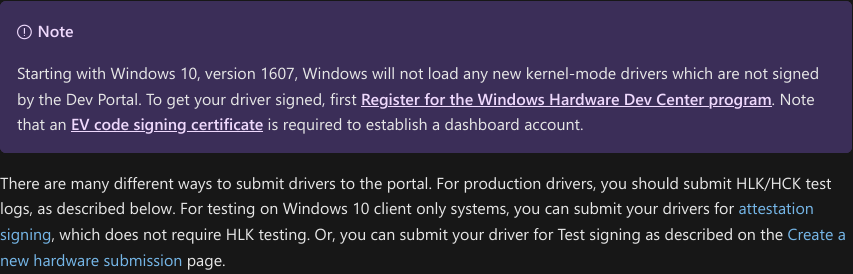
\includegraphics[width=\textwidth]{../antianti/window-driver-sign}}{
    Note: \textLF
    Starting with Windows 10, version 1607, Windows will not load any new kernel-mode drivers which are
    not signed by the Dev Portal. To get your driver signed, first Register for the Windows Hardware Dev
    Center program. Note that an EV code signing certificate is required to establish a dashboard account.
    \textLF\textLF
    There are many different ways to submit drivers to the portal. For production drivers, you should submit
    HLK/HCK test logs, as described below. For testing on Windows 10 client only systems, you can submit your
    drivers for attestation signing, which does not require HLK testing. Or, you can submit your driver for
    Test signing as described on the Create a new hardware submission page.
}
\end{frame}

\begin{frame}{Window driver key stealing}
\pdftooltip{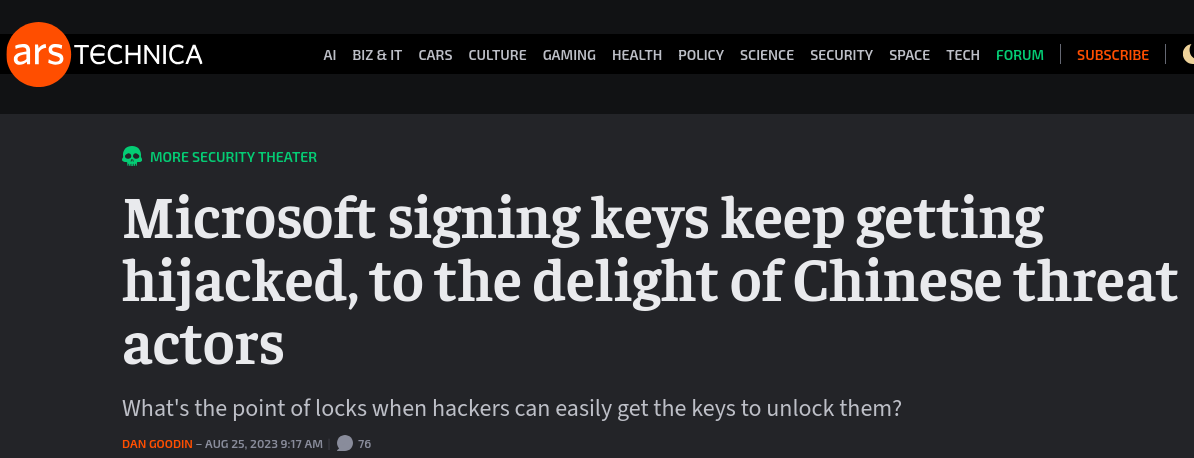
\includegraphics[width=\textwidth]{../antianti/window-driver-sign-steal}}{
Headline on ArsTechnica dated Aug 25, 2023  with byline by Dan Goodin.\textLF\textLF
Microsoft singing keys keep getting hijacked, to the delight of Chinese threat actors\textLF
What's the point of locks when hackers can easily get the keys to unlock them?
}
\end{frame}

\begin{frame}{aside: driver or not driver?}
    \begin{itemize}
    \item why does random device driver have permission to do all these `hiding' operations?
    \vspace{.5cm}
    \item (if you've taken CSO2) kernel mode $\rightarrow$ full hardware access
    \item there are OS designs where drivers don't run with full access
        \begin{itemize}
        \item but real performance/complexity costs
        \end{itemize}
    \end{itemize}
\end{frame}

\begin{frame}{chkrootkit}
    \begin{itemize}
    \item \texttt{chkrootkit} --- Unix program that looks for rootkit signs
    \vspace{.5cm}
    \item tell-tale strings in system programs
        \begin{itemize}
        \item e.g. file, process, network connection listing programs changed
        \end{itemize}
    \item disagreement between process list, other ways of detecting processes
    \item disagreement between file lists, other ways of counting files
    \item overwritten entries in system login records
    \item known suspicious filenames
        \begin{itemize}
        \item hidden exes in temporary, data directories, etc.
        \end{itemize}
    \end{itemize}
\end{frame}
